\section{Experiments}
\label{sec:experiments}

\subsection{Experimental setup}
\noindent\textbf{Implementation Details. }To ensure a fair comparison, we adopt the protocol of \citep{zhang2023vqacl} for both feature extraction and training across datasets. For the visual embeddings, we use a Faster R-CNN~\citep{faster_rcnn} trained on the Visual Genome dataset~\citep{Krishna2016VisualGC} extracting 36 region-based object features per image in the VQAv2 dataset. For videos in the NExT-QA dataset, we extract clip-level motion features using an inflated 3D ResNeXt-101~\citep{hara3dcnns}, setting $n = 16$ regions per clip. A two-layer MLP with GELU activation adapts these features for input into the transformer backbone. Our transformer backbone, based on T5~\citep{2020t5}, consists of 12 blocks for both encoder and decoder modules, each containing 12 attention heads. The embedding dimension $d$ is tailored to the task-specific requirements. Training is conducted for 3 epochs per task, with a batch size of 80. We utilize the Adam optimizer~\citep{KingBa15} with an initial learning rate of $10^{-4}$. $\lambda$ is set to $0.5$ in all experiments. All implementations are based on PyTorch~\citep{pytorch}. Importantly, unlike~\citep{zhang2023vqacl}, \qstmethodshort{} does not store any visual or question prototypes.


\noindent\textbf{Evaluation Metrics. }We utilise two established metrics for continual learning~\citep{zhang2023vqacl, Chaudhry_2018, lopezpaz2022gradientepisodicmemorycontinual}: final average performance ($AP$), and average forgetting ($Forget$). The $AP$ metric reflects the model's overall performance across all learnt tasks, highlighting its ability to consistently acquire new tasks. Let $a_{i,j}$ represent the performance of the model on task $\mathcal{T}^i$ after it has completed learning this task $\mathcal{T}^j$. Then, $AP$ is calculated as: $AP\!=\!\frac{1}{T} \sum_{t=1}^{T} a_{t,T}.$
Additionally, the $Forget$ metric serves as a proxy for knowledge retention, quantifying performance degradation on prior tasks as new tasks are learned. It is computed as:
$Forget\!=\!\frac{1}{T-1} \sum_{t=1}^{T-1} \max_{z \in \{t, \ldots, T-1\}} (a_{t,z} - a_{t,T}).$ To ensure a fair comparison, For NExT-QA, following \citep{zhang2023vqacl, xiao2021next}, we compute $a_{i,j}$ using Wu-Palmer Similarity (WUPS) to evaluate answer quality. For the VQAv2 dataset, as described in \citep{zhang2023vqacl}, we use the percentage of correctly answered questions as the value for $a_{i,j}$.\\
\noindent\textbf{Baselines. }We benchmark \qstmethodshort{} against five established continual learning methods spanning regularization and rehearsal-based strategies. This includes two regularization-based methods: Elastic Weight Consolidation (EWC)~\citep{kirkpatrick2017overcoming} and Memory Aware Synapses (MAS)~\citep{mas2018}, as well as three rehearsal-based approaches: Experience Replay (ER)~\citep{chaudhry2019tinyepisodicmemoriescontinual}, Dark Experience Replay (DER)~\citep{Chaudhry2019er}, Virtual Sample (VS)~\citep{Wan_2022_CVPR}, and VQACL~\citep{zhang2023vqacl} (see details in Appendix). We additionally report lower and upper performance bounds to frame the results: a lower bound (Vanilla) using naive finetuning without forgetting mitigation, and an upper bound (Joint) that trains on all tasks simultaneously. Following the evaluation protocol in VQACL~\citep{zhang2023vqacl}, we employ two key evaluation strategies: standard testing, which evaluates the models' performance on previously encountered task types, assessing their ability to retain learnt knowledge, and novel composition testing, which challenges the models with previously unseen combinations of visual and linguistic elements, probing their capacity for compositional  generalization. This twofold evaluation reveals how well each method balances retention and adaptation (details in Appendix). Additional experiments using pretrained models are included in the Supp Mat.

\input{sec/tables/novel_tab}

\subsection{Main results}
\label{sec:mainresults}
\noindent\textbf{Performance Analysis On Standard Setting. }Tab.~\ref{tab:model_performance} shows a detailed comparison of continual learning approaches in the VQACL setting, with our proposed \qstmethodshort{} achieving superior performance across both standard and novel composition tests. \qstmethodshort{} consistently outperforms other methods in AP and forgetting demonstrating robust knowledge retention. On VQAv2, \qstmethodshort{} attains an AP of 39.25\% in standard testing, outperforming the best rehearsal-based approach (VQACL) by 1.79\%. Similarly, in NExT-QA, \qstmethodshort{} achieves an AP of 31.70\%, exceeding competing methods by 0.84\% to 4.73\%. The forgetting rates for \qstmethodshort{} are also the lowest, with 4.91\% and 2.91\% for VQAv2 and NExT-QA, respectively, underscoring its capacity for stable knowledge retention.

In novel composition testing, \qstmethodshort{} demonstrates strong generalization, achieving top AP scores of 40.00\% on VQAv2 and 33.85\% on NExT-QA. Notably, despite not storing images, our approach maintains high performance in novel settings, with a minimal performance gap between standard and novel composition tests (0.75\% for VQAv2 and 0.64\% for NExT-QA). This narrow gap indicates that distilling knowledge using only seen questions effectively reinforces visual-linguistic associations, enabling the model to generalise well even in unfamiliar contexts. This performance underscores \qstmethodshort{}'s capacity to construct robust, adaptable representations, showing that question-only distillation can successfully support compositional reasoning without the need for visual memory.

\noindent\textbf{Performance Analysis of Novel Composition Testing. }Tab.~\ref{tab:vqa_performance} provides a detailed comparison of model performance on novel and seen skill-concept compositions across VQAv2 and NExT-QA datasets. \qstmethodshort{} consistently surpasses previous approaches. On VQAv2, \qstmethodshort{} shows significant gains over VQACL, with an average improvement of 4.60\% on novel compositions and 3.81\% on seen compositions. This result indicates enhanced compositional generalisation, as evidenced by the smaller gap between novel and seen performance compared to other methods. For NExT-QA, \qstmethodshort{} maintains competitive performance, with slight gains over VQACL on seen groups (average +0.27\%) in a dataset that presents unique challenges, such as temporal and causal reasoning. For such tasks, storing images may be necessary to maintain a comprehensive task understanding. These consistent gains highlight \qstmethodshort{}'s robustness in compositional reasoning, validating its effectiveness for continual VQA. 

\section{Ablation Study and Analysis}
\label{sec:ablation}
\begin{figure*}[ht]
    \centering
    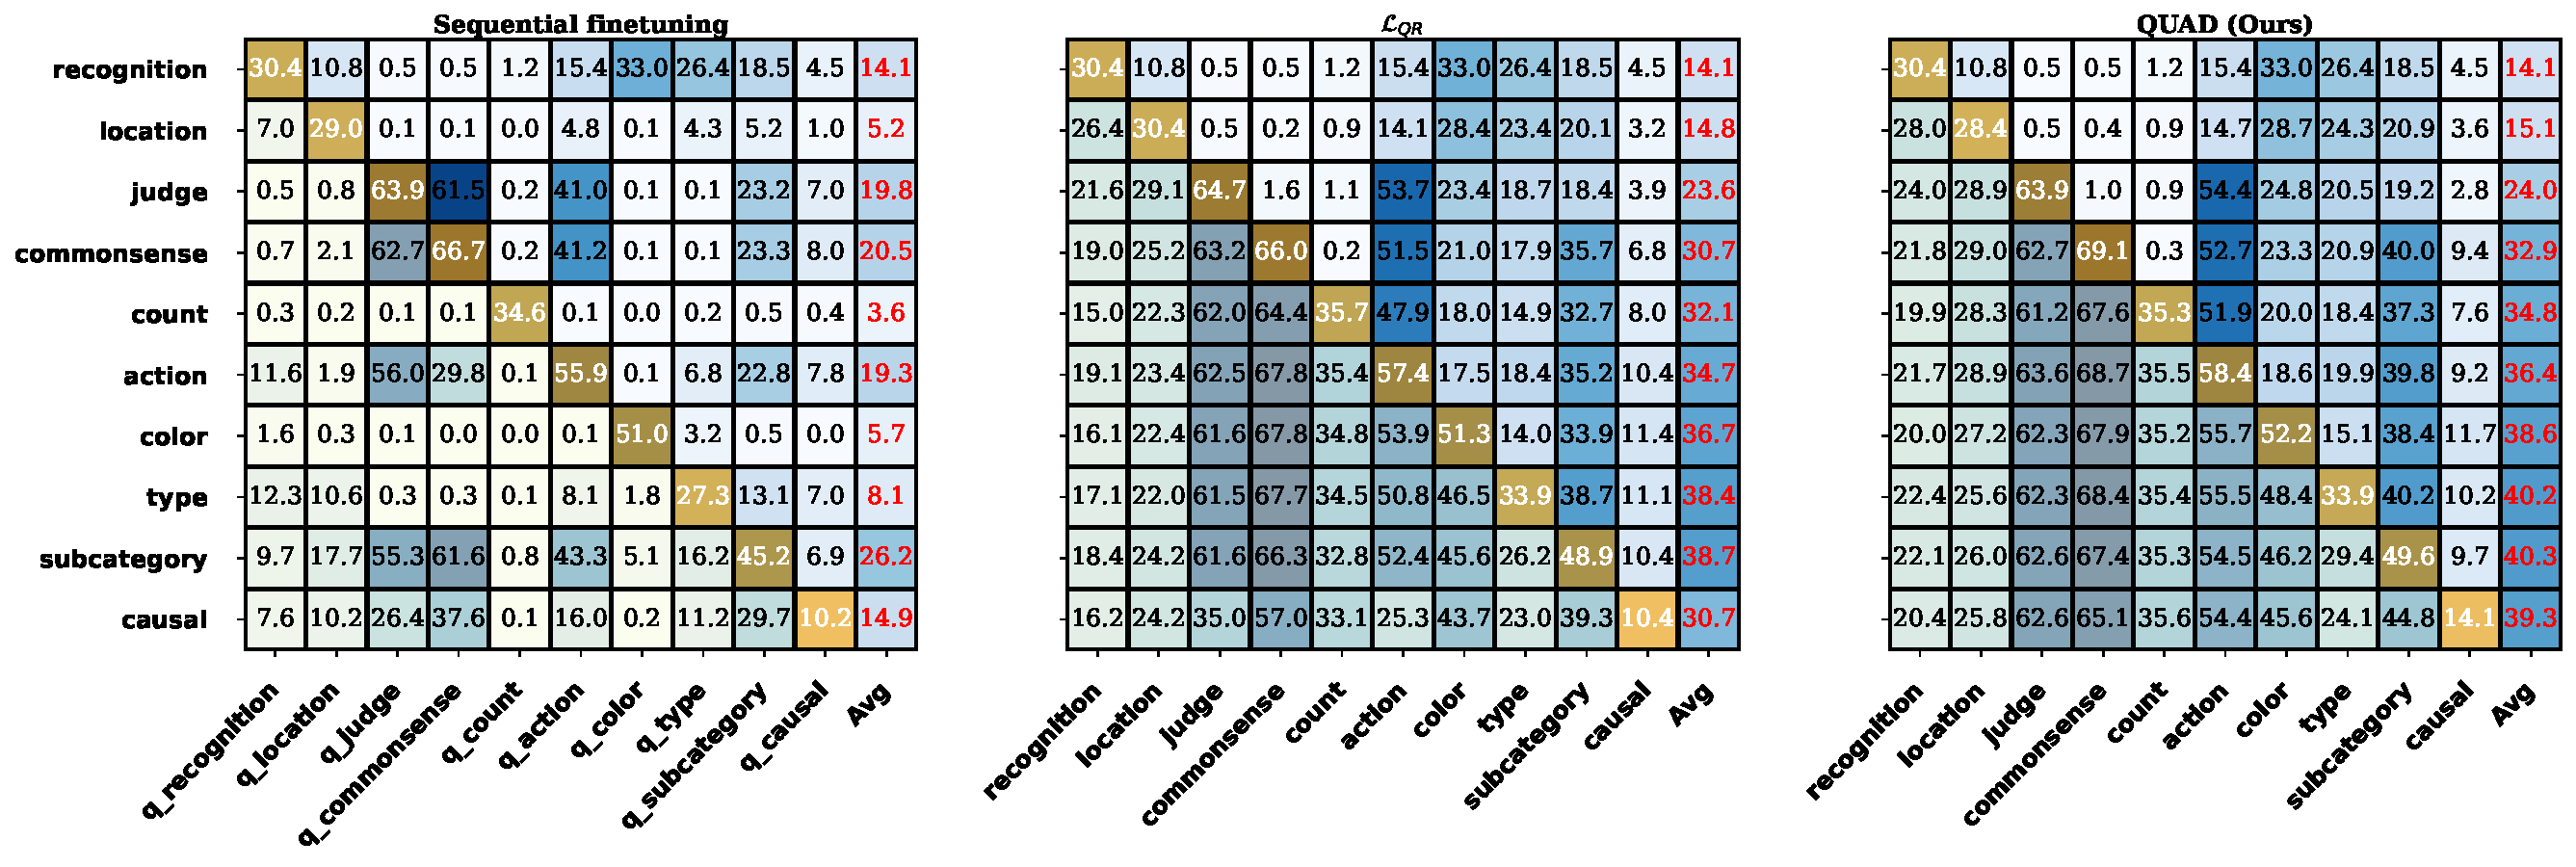
\includegraphics[width=\textwidth]{Figures/matrix_plots_vqa.pdf}
    \vspace{-8mm}
    \caption{\textbf{Plasticity/Stability analysis on VQAv2. }Each matrix shows the performance of a model trained on tasks (rows) and evaluated on tasks \textbf{sequentially} (columns). The diagonal (highlighted in {\color{orange}{orange}}) represents in-domain performance, while off-diagonal elements indicate cross-domain generalization. Higher values (darker colors) suggest better retention and plasticity. The progression from `Sequential finetuning', to $\mathcal{L}_{QR}$ and then to our full method, QUAD, highlights the improvement in retaining knowledge across sequential tasks.}
    \vspace{-3mm}
    \label{fig:cross_task_generalization}
\end{figure*}

\noindent \circled{1} \noindent\textbf{\qstmethodshort{} Components. }Tab.~\ref{tab:comparison_distillation} shows the impact of questions-only replay and attention distillation in \qstmethodshort{}. We evaluate: (1) \textit{Question-only replay alone}, (2) \textit{attention distillation alone}, and (3) \textit{the combination of both}.

Using question-only replay mechanism achieves moderate performance, with AP of 30.72\% on VQAv2 and 29.04\% on NExT-QA, indicating effective knowledge preservation across tasks. In contrast, attention distillation alone yields lower AP scores (13.34\% on VQAv2 and 13.24\% on NExT-QA) with high forgetting scores (32.08\% on VQAv2 and 24.56\% on NExT-QA), suggesting limited task adaptation. Combining $\mathcal{L}_{\text{QR}}$ and $\mathcal{L}_{\text{ACD}}$ achieves the best results, with AP scores of 39.25\% on VQAv2 and 31.70\% on NExT-QA, and the lowest forgetting rates.

\noindent \circled{2} \textbf{Attention Distillation. }Tab.~\ref{tab:attn_distillation} demonstrates the effectiveness of our proposed {$\mathcal{L}_{\text{ACD}}$} within \qstmethodshort{}. Unlike prior methods such as Attn-dist (L1) and Asym-Attn~\citep{pelosin2022towards}, which impose L1 or ReLU+L1 losses on raw attention scores, our approach applies cross-entropy over normalized attention maps. \qstmethodshort{} outperforms previous methods, achieving an AP of 39.25\% and Forgetting of 4.91\% on VQAv2, and an AP of 31.70\% with Forgetting of 2.91\% on NExT-QA. These results highlight the benefit of distributional consistency in attention maps over unstructured alignment.
\begin{table}[t]
    \centering
    \caption{Ablation study of \qstmethodshort{} components.} %on VQAv2 and NExT-QA.}
    \vspace{-3mm}
    \renewcommand{\arraystretch}{1.2}
    \setlength{\tabcolsep}{8pt}
    \resizebox{0.48\textwidth}{!}{%
    \begin{tabular}{c|c|c|cc|cc}
    \toprule
    \multirow{2}{*}{$\mathcal{L}_{\text{QR}}$} & \multirow{2}{*}{$\mathcal{L}_{\text{ACD}}$} & \multirow{2}{*}{\textbf{Memory}} & \multicolumn{2}{c|}{\textbf{VQAv2}} & \multicolumn{2}{c}{\textbf{NExT-QA}} \\ 
    \cline{4-7} 
    & & \textbf{Type} & \textbf{AP (↑)} & \textbf{Forget (↓)} & \textbf{AP (↑)} & \textbf{Forget (↓)} \\
    \midrule
    $\checkmark$ &  & \faQuestionCircle & 30.72 & 13.74 & 29.04 & 4.58 \\
    & $\checkmark$ & \faQuestionCircle & 13.34 & 32.08 & 13.24 & 24.56 \\
    $\checkmark$ & $\checkmark$ & \faQuestionCircle & \textbf{39.25} & \textbf{4.91} & \textbf{31.70} & \textbf{2.91} \\ 
    \bottomrule
    \end{tabular}
    }
    \vspace{-3mm}
    \label{tab:comparison_distillation}
\end{table}
\begin{table}[t]
    \centering
    \caption{Comparison of attention distillation methods.}
    \vspace{-3mm}
    \renewcommand{\arraystretch}{1.2}
    \setlength{\tabcolsep}{8pt}
    \resizebox{0.48\textwidth}{!}{%
    \begin{tabular}{c|cc|cc}
    \toprule
    \multirow{2}{*}{\textbf{Method}} & \multicolumn{2}{c|}{\textbf{VQAv2}} & \multicolumn{2}{c}{\textbf{NExT-QA}} \\
    & \textbf{AP (↑)} & \textbf{Forget (↓)} & \textbf{AP (↑)} & \textbf{Forget (↓)} \\
    \midrule
    $\mathcal{L}_{\text{QR}}$ + Attn-dist (L1) & 34.56 & 7.91 & 30.14 & 5.78 \\
    $\mathcal{L}_{\text{QR}}$ + Asym-Attn \citep{pelosin2022towards} & 38.15 & 5.57 & 31.18 & 4.13\\
    \cmidrule{1-5}
    \textbf{\qstmethodshort{} (Ours)} & \textbf{39.25} & \textbf{4.91} & \textbf{31.70} & \textbf{2.91} \\ 
    \bottomrule
    \end{tabular}
    }
    \vspace{-3mm}
    \label{tab:attn_distillation}
\end{table}

\noindent \circled{3} \textbf{Analysing Plasticity/Stability. }Fig.~\ref{fig:cross_task_generalization} compares how different methods manage forgetting and adaptation on the VQAv2 dataset. The sequential fine-tuning baseline (left) exhibits uniformly low off-diagonal scores, signaling a complete failure to retain knowledge from earlier tasks. This severe forgetting stems from overfitting to the current task’s answer space, a phenomenon we call the \textit{out-of-answer-set problem}, it occurs when the model overfits to the current task’s answer space, preventing it from correctly responding to questions from earlier tasks. By contrast, question-only replay $\mathcal{L}_{\text{QR}}$ (center) noticeably improves retention through our question-only replay mechanism, especially in tasks like ``commonsense'' and ``count''. However, it remains less effective in complex reasoning tasks like ``causal'' and ``subcategory''. 

Our full method, \qstmethodshort{} (right), achieves the best balance: it sustains high diagonal accuracy while boosting off-diagonal retention. reflecting both adaptability and long-term memory. For example, \qstmethodshort{} preserves 62.6\% accuracy on the `judge' task, compared to only 35.0\% with replay alone—highlighting the value of attention consistency distillation. Notably, tasks like `type' that rely heavily on visual semantics remain challenging under the question-only setting, reaffirming the need for richer visual grounding in some categories. Nevertheless, \qstmethodshort{} excels in conceptually driven tasks such as ``commonsense'', showing its effectiveness even with reduced supervision.

\noindent \circled{4} \textbf{Sensitivity to Memory Size. }Fig.~\ref{fig:memory_size_comparison} shows how different continual learning methods respond to varying memory budgets. Across all memory sizes, \qstmethodshort{} consistently outperforms baselines (ER, DER, VS, VQACL), demonstrating the effectiveness of our distillation strategy. On VQAv2, \qstmethodshort{} exhibits robust scalability, with AP increasing steadily from 1K to 5K samples. In constrained storage scenarios, \qstmethodshort{} maintains competitive performance by leveraging question-only distillation. On the more visually complex NExT-QA benchmark, \qstmethodshort{} still leads, though with narrower margins. This reflects the greater challenge of retaining visual-semantic alignment using question-only signals.
\begin{figure}[t]
\centering
        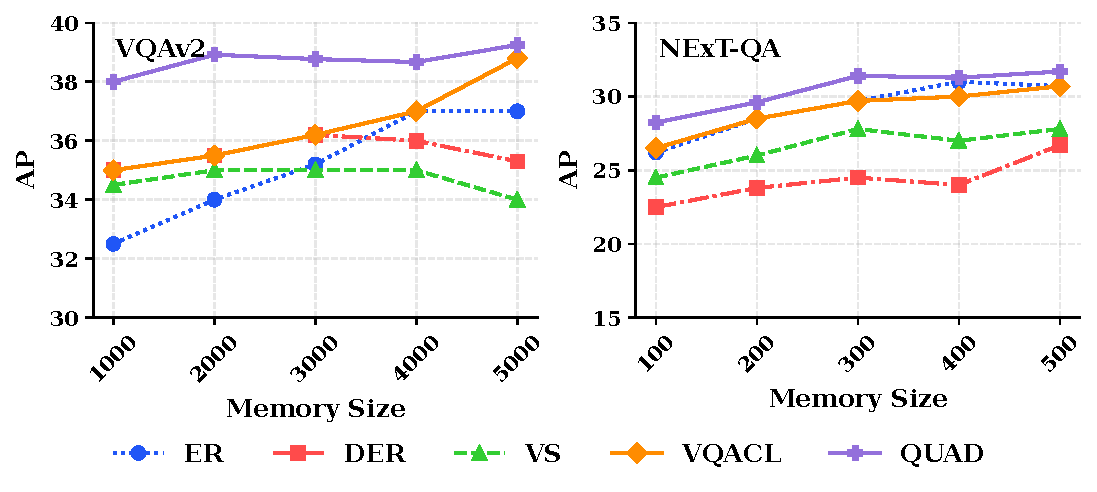
\includegraphics[width=\linewidth]{Figures/memory_size_effect.pdf}
        \caption{\textbf{Sensitivity analysis to memory size}. Our method, \qstmethodshort{}, consistently achieves higher AP than baselines, demonstrating strong scalability on VQAv2 and stable performance on NExT-QA, especially as memory size increases.}
        \label{fig:memory_size_comparison}
\end{figure}

\noindent \circled{5} \textbf{Effectiveness of Object-Matched Question Selection. }Fig.~\ref{fig:random_vs_obj} highlights the advantage of object-matched question selection compared to random pairing. We analyze its impact across memory sizes on VQAv2 and NExT-QA, where it consistently improves AP as memory grows. This targeted selection ensures semantic relevance between the question and visual context, which helps reinforce meaningful cross-task associations. As a result, the model adapts effectively to new tasks while retaining prior knowledge.
\definecolor{mediumpurple}{HTML}{9370DB}
\begin{figure}
    \centering
    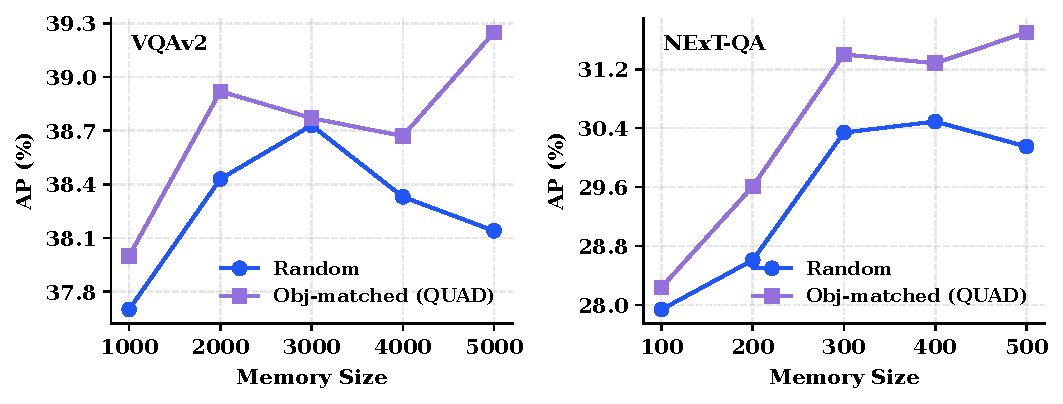
\includegraphics[width=\linewidth]{Figures/random_performance_comparison.pdf}
    \caption{\textbf{Question selection strategy in \qstmethodshort{}}. Figure shows AP for random (\textcolor{blue}{blue}) and object-matched (\textcolor{mediumpurple}{purple}) question selection across memory sizes on VQAv2, and NExT-QA. Object-matched selection consistently outperforms random selection.}
    \label{fig:random_vs_obj}
\end{figure}